
{\section{Trajectory Aging}}
\label{sec-aging}

Suppose that we have compressed a trajectory $\dddot{\mathcal{T}_0}$ to $\overline{\mathcal{T}}_1$ using any \lsa algorithm $\mathcal{A}$ with an error bound $\epsilon_1$. As time evolves, we may need to further compress $\overline{\mathcal{T}}_1$ to an even coarser trajectory $\overline{\mathcal{T}}_2$.
What is the relationship among $\overline{\mathcal{T}}_2$, $\overline{\mathcal{T}}_1$ and $\dddot{\mathcal{T}_0}$? And what is the right way to get the coarser trajectory $\overline{\mathcal{T}}_2$?
\myblue{What line simplification algorithms should we use in the first and second rounds of simplifications? If the first round of simplification uses algorithm $A_1$, can we use algorithm $A_2$ in the second round? How to set the parameter of error bounds in these simplifications? And after multiple rounds of simplifications, does the coarse trajectory still have bounded errors \wrt the original trajectory?}
%
This section is to answer these questions from the views of friendliness \cite{Cao:Spatio} (Section \ref{sec-aging-friend}) and errors (Section \ref{sec-aging-safe}).
Note that (1) if we get $\overline{\mathcal{T}}_1$ and $\overline{\mathcal{T}}_2$ by optimal algorithms \wrt error bounds $\epsilon_1$ and $\epsilon_2$, respectively, then $\overline{\mathcal{T}}_2$ may not be the optimal one of $\dddot{\mathcal{T}_0}$ \wrt any error bound \cite{Cao:Spatio}, \textcolor{blue}{and (2) as \lissed is a special case of \sed, we refer to the \sed errors rather than the \lissed errors when we talk about aging friendliness and errors of algorithms using \lissed (recall that \emph{if the \lissed error bound of such an algorithm  is set to $\epsilon^2$, then its maximal \sed error is not greater than $\epsilon$})}. The major results are summarized in \mytable{tab:summary-data-aging}.
%Hence, we focus on sub-optimal error bounded trajectory simplification algorithms only.


\subsection{Friendliness of Data Aging}
\label{sec-aging-friend}
We first discuss the relationship between $\overline{\mathcal{T}}_1$ and $\overline{\mathcal{T}}_2$ from the view of friendliness, which was defined in \cite{Cao:Spatio}, but was seldom discussed later.
	
\stitle{Aging friendly \cite{Cao:Spatio}}. {An \lsa algorithm $\mathcal{A}$ is aging friendly with respect to a distance metric $\mathcal{M}$ if for every $\epsilon_1$ and every $\epsilon_2$ such that $\epsilon_1 < \epsilon_2$, and for every trajectory $\dddot{\mathcal{T}}$, $\mathcal{A}(\dddot{\mathcal{T}}, \epsilon_2, \mathcal{M})= \mathcal{A}(\mathcal{A}(\dddot{\mathcal{T}}, \epsilon_1, \mathcal{M}), \epsilon_2, \mathcal{M})$.}

Cao et al. proved in \cite{Cao:Spatio} that ``an optimal line simplification algorithm is not aging-friendly \wrt~the \ped and \sed'', and ``the top-down algorithm \dpa is aging friendly \wrt~\ped and \sed'' on the premise that the second run of \dpa takes as input the whole simplified trajectory produced by the first run.
However, algorithms other than the optimal algorithms and the top-down algorithm \dpa with distance metrics other than \ped and \sed are not discussed in \cite{Cao:Spatio}, thus, their effectiveness in data aging remains an open problem.
In the rest, we  present a full picture of this problem, starting from the optimal algorithms coupling with \dad.

\begin{table}
	\renewcommand{\arraystretch}{1.20}
	\vspace{-1ex}
	\caption{\small Aging friendliness and error bounds of line simplification algorithms for data aging}
	\label{tab:summary-data-aging}
	\centering
	\scriptsize
	\begin{tabular}{|c|c|c|c|c|}
		\hline
		{\bf{Algorithms}} &\bf{Distance Metrics} & \bf{Aging Friendliness} &  {\bf{Error Bounds}}  \\		
		\hline

		{\multirow{2}*{{\opt} algorithms}} &\ped or \sed	& \hspace{2ex} $\times$ (\cite{Cao:Spatio})  & $\epsilon_1 + \epsilon_2$  (Prop. \ref{theo-aging-distance})	\\
		\cline{2-4}
		
		&\dad	& $\times$  (Prop. \ref{theo-aging-opt-dad}) &$\epsilon_1 + \epsilon_2$  (Prop. \ref{theo-aging-distance})\\
		\hline
		
		{\multirow{2}*{Batch algorithm \dpa}} &\ped or \sed	&\checkmark (\cite{Cao:Spatio})  & $\max(\epsilon_1, \epsilon_2)$   (Prop. \ref{theo-aging-error-dp})\\
		\cline{2-4}
		
		&\dad	& $\times$  (Prop. \ref{theo-aging-dp-dad})  & $\epsilon_1 + \epsilon_2$   (Prop. \ref{theo-aging-distance})\\
		\hline
		
		{Batch algorithm \tpa}	& \ped, \sed or \dad & $\times$  (Prop. \ref{theo-aging-tp})  &$\epsilon_1 + \epsilon_2$  (Prop. \ref{theo-aging-distance})  \\
		\hline
		
		{Online algorithms}	& \ped, \sed or \dad & $\times$  (Prop. \ref{theo-aging-online}) &$\epsilon_1 + \epsilon_2$  (Prop. \ref{theo-aging-distance})  \\
		\hline

		{One-pass algorithms}	& \ped, \sed or \dad & $\times$ (Prop. \ref{theo-aging-online}) &$\epsilon_1 + \epsilon_2$  (Prop. \ref{theo-aging-distance})  \\

		\hline
	\end{tabular}
	\vspace{-2ex}
\end{table}




\begin{proposition}
	\label{theo-aging-opt-dad}
	An optimal algorithm is not aging friendly \wrt~\dad too.
\end{proposition}

\begin{proof}
	We shall prove this by constructing a counter-example shown in Figure~\ref{fig:aging-opt-dad}, where error bounds $\epsilon_1 =30^o$ and $\epsilon_2=45^o$.
	
	\underline{(1) ${\opt}(\dddot{\mathcal{T}}, 45^o, \dad)$}.
	It first constructs the reachability graph of the trajectory that $P_0$ has arcs to $P_1$ and $P_2$, $P_1$ has arcs to $P_2$ and $P_3$, and $P_2$ has an arc to $P_3$. At last, it outputs a shortest path of three points $\{P_0, P_2, P_3\}$.
	
	\underline{(2) ${\opt}(\opt(\dddot{\mathcal{T}}, 30^o, \dad), 45^o, \dad)$}. In the first round ($\epsilon_1=30^o$), the original trajectory is compressed to three points $\{P_0, P_2, P_3\}$, and in the second round ($\epsilon_2=45^o$), because line segments  $\overline{P_0P_2}$ and $\overline{P_2P_3}$ both have angular deviations to line segment $\overline{P_0P_3}$ less than $45^o$, it is finally compressed to two points $\{P_0, P_3\}$.
	
	In this case, ${\opt}(\dddot{\mathcal{T}}, 45^o, \dad) \ne {\opt}(\opt(\dddot{\mathcal{T}}, 30^o, \dad), 45^o, \dad)$. Thus, algorithm \opt is not aging friendly \wrt~\dad.
\end{proof}	
	
\begin{figure}
		\centering
		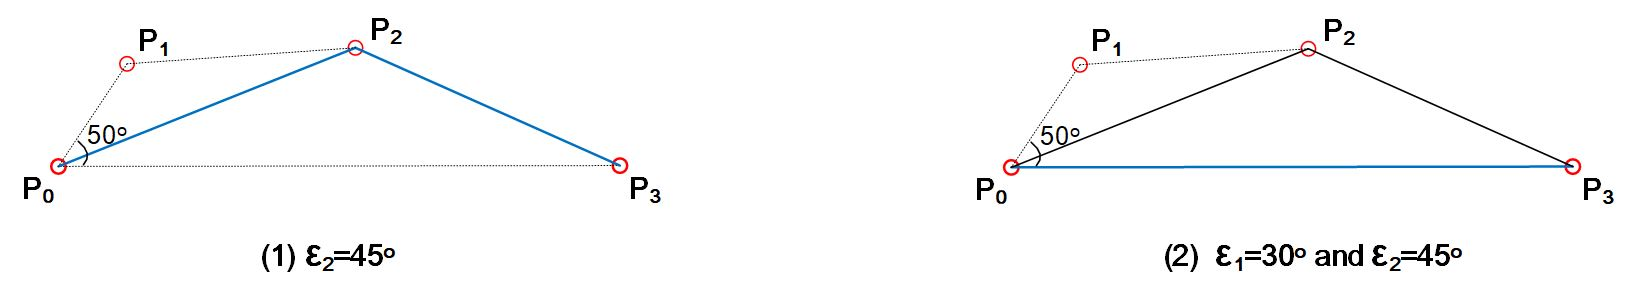
\includegraphics[scale=0.68]{Figures/Fig-aging-opt.jpg}
		
		\caption{\small A counter example of the aging friendliness of algorithm \opt using \dad, where (1) the original trajectory $\{P_0, P_1, P_2, P_3\}$ is compressed using $\epsilon_2=45^o$ to three points $\{P_0, P_2, P_3\}$, and (2) it is first compressed using $\epsilon_1=30^o$ to three points $\{P_0, P_2, P_3\}$, then compressed using $\epsilon_2=45^o$ to two points $\{P_0, P_3\}$. }
		\vspace{-1ex}
		\label{fig:aging-opt-dad}
\end{figure}

%%%%%%%%%%%%%%%%%%%%%%%% DP + DAD

\begin{proposition}
	\label{theo-aging-dp-dad}
	The top-down algorithm \dpa is not aging friendly \wrt~\dad.
\end{proposition}

\begin{proof}
	We shall prove this by constructing a counter-example shown in Figure~\ref{fig:aging-dp-dad}, where error bounds $\epsilon_1 =30^o$ and $\epsilon_2=45^o$.
	
	\underline{(1) ${\dpa}(\dddot{\mathcal{T}}, 45^o, \dad)$}. It finds that line segment $\overline{P_1P_2}$ has the largest angular deviation to line segment $\overline{P_0P_4}$ which is also larger than the error bound $45^o$, hence it uses point $P_2$ as the splitting point and splits the original trajectory to $\{P_0, P_1, P_2\}$ and $\{P_2, P_3, P_4\}$. At last, it outputs three points $\{P_0, P_2, P_4\}$.
	
	\underline{(2) ${\dpa}(\dpa(\dddot{\mathcal{T}}, 30^o, \dad), 45^o, \dad)$}. In the first round ($\epsilon_1=30^o$), the original trajectory is compressed to three points $\{P_0, P_2, P_4\}$, and in the second round ($\epsilon_2=45^o$), because line segments  $\overline{P_0P_2}$ and $\overline{P_2P_4}$ both have angular deviations to line segment $\overline{P_0P_4}$ less than $45^o$, it is finally compressed to two points $\{P_0, P_4\}$.
	
	In this case, ${\dpa}(\dddot{\mathcal{T}}, 45^o, \dad) \ne {\dpa}(\dpa(\dddot{\mathcal{T}}, 30^o, \dad), 45^o, \dad)$. Thus, the \dpa algorithm is not aging friendly \wrt~\dad.
\end{proof}

\begin{figure}
	\centering
	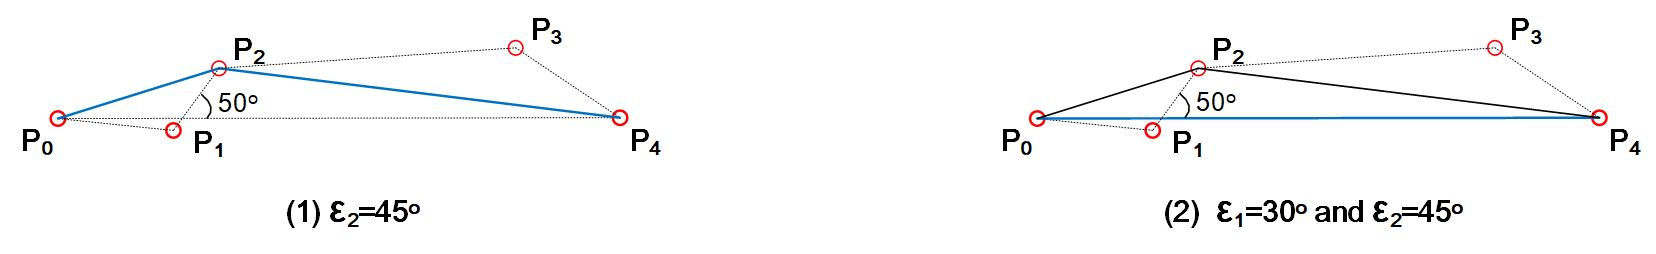
\includegraphics[scale=0.66]{Figures/Fig-aging-dp.jpg}
	
	\caption{\small A counter example of the aging friendliness of \dpa using \dad, where (1) the original trajectory is compressed using $\epsilon_2=45^o$ to three points $\{P_0, P_2, P_4\}$, and (2) the original trajectory is first compressed using $\epsilon_1=30^o$ to three points $\{P_0, P_2, P_4\}$, then compressed using $\epsilon_2=45^o$ to two points $\{P_0, P_4\}$. }
	\vspace{-1ex}
	\label{fig:aging-dp-dad}
\end{figure}

The \dpa using \dad is different with \ped and \sed in that \dad is the deviation between two line segments rather than the deviation between a point and a line segment. For example, in Figure \ref{fig:aging-dp-dad}-(2), the angular deviations of line segments $\overline{P_1P_2}$ and $\overline{P_0P_2}$ to line segment $\overline{P_0P_4}$ are certainly different though they pass through the same point $P_2$, thus, in the first round of run ($\epsilon_1=30^o$), the point $P_2$ serves as a splitting point while in the second round of run ($\epsilon_2=45^o$), it is no more a splitting point. This difference is the key that lets \dpa using \dad not aging friendly.
%
We next discuss the aging friendliness of other algorithms.

\begin{figure}
	\centering
	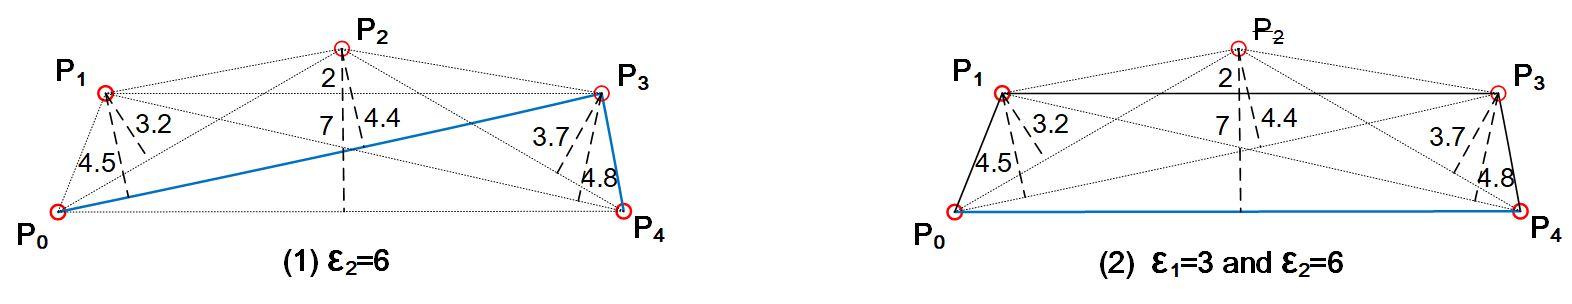
\includegraphics[scale=0.66]{Figures/Fig-aging-pavlidis.jpg}

	\caption{\small A counter example of the aging friendliness of algorithm \tpa, where (1) the original trajectory is compressed using $\epsilon_2=6$ to three points $\{P_0, P_3, P_4\}$, and (2) the original trajectory is first compressed using $\epsilon_1=3$ to four points $\{P_0, P_1, P_3, P_4\}$, then compressed using $\epsilon_2=6$ to two points $\{P_0, P_4\}$. }
	\vspace{-1ex}
	\label{fig:aging-pavlidis}
\end{figure}


\begin{proposition}
\label{theo-aging-tp}
The bottom-up algorithm \tpa is not aging friendly \wrt~\ped, \sed or \dad.
\end{proposition}

\begin{proof}
	We shall prove this by constructing a counter-example shown in Figure~\ref{fig:aging-pavlidis}, where error bounds $\epsilon_1 =3$ and $\epsilon_2=6$, and without losing generality, we use \ped as the distance metric.

\underline{(1) ${\tpa}(\dddot{\mathcal{T}}, 6, \ped)$}. It first merges $\overline{P_1P_2}$ and $\overline{P_2P_3}$ to $\overline{P_1P_3}$ as the merging of them has the lowest cost of $2$, the distance from point $P_2$ to line segment $\overline{P_1P_3}$; then it merges $\overline{P_0P_1}$ and $\overline{P_1P_3}$ to $\overline{P_0P_3}$ with the lowest cost of $4.5$, the distance from point $P_1$ to line segment $\overline{P_0P_3}$; at last, because the merging of $\overline{P_0P_3}$ and $\overline{P_3P_4}$ has a cost of $7$, the distance from point $P_2$ to line segment $\overline{P_0P_4}$, which is larger than the error bound of $6$, it outputs three points $\{P_0, P_3, P_4\}$.

\underline{(2) ${\tpa}(\tpa(\dddot{\mathcal{T}}, 3, \ped), 6, \ped)$}. In the first round ($\epsilon_1=3$), the original trajectory is compressed to four points $\{P_0, P_1, P_3, P_4\}$, and in the second round ($\epsilon_2=6$), because all points in the result trajectory $\{P_0, P_1, P_3, P_4\}$ have distances to line segment $\overline{P_0P_4}$ less than $6$, it is finally compressed to two points $\{P_0, P_4\}$.

In this case, ${\tpa}(\dddot{\mathcal{T}}, 6, \ped) \ne {\tpa}(\tpa(\dddot{\mathcal{T}}, 3, \ped), 6, \ped)$. Thus, \tpa is not aging friendly \wrt~\ped.
Similarly, \tpa is not aging friendly \wrt~ \sed or \dad. Hence, we have the conclusion.
\end{proof}


\eat{%%%%%%%%%%%%%
\begin{proposition}
	\label{theo-aging-squishe}
	The online algorithm \squishe is not aging friendly \wrt~\sed.
\end{proposition}

\begin{proof}
	\textcolor{blue}{(In brief) The \squishe algorithm runs in a bottom-up manner that is a slight variation of algorithm \tpa. As \tpa, it is not aging friendly \wrt~\sed.}
\end{proof}
}%%%%%%%%%%%%%%%%
	
\begin{figure}[tb!]
	\centering
	\includegraphics[scale=0.66]{Figures/Fig-aging-incre.jpg}
	\vspace{-1ex}
	\caption{\small Counter examples of the aging friendliness of incremental algorithms (either online or one-pass).}
	\vspace{-1ex}
	\label{fig:aging-incre}
\end{figure}

\begin{proposition}
	\label{theo-aging-online}
	The online and one-pass algorithms are not aging friendly \wrt \ped, \sed or \dad.

\end{proposition}

\begin{proof}
	For online algorithm \squishe, it supports \sed only and runs in a bottom-up manner that is a slight variation of algorithm \tpa. As \tpa, it is not aging friendly \wrt~\sed.
	For other online and one-pass algorithms, though they apply different distance checking approaches, they run in a common incremental manner, \ie they incrementally read data points until they can not represent those read points by one line segment, then they output the simplified sub-trajectory and continue to process the rest data points. We next construct counter examples to show that an incremental algorithm $\mathcal{A}$ is not aging friendly.
	
	\underline{(1) ${\mathcal{A}}(\dddot{\mathcal{T}}, \epsilon_2, \mathcal{M})$}. As shown in Figure~\ref{fig:aging-incre}-(1)(3)(5), the algorithm $\mathcal{A}$ incrementally reads $\{P_0, P_1,\dddot, P_5\}$ and finds they can be represented by line segment $\overline{P_0P_4}$, thus the process progresses. Then, after point $P_6$ is read, it finds that these points can not be represented by any line segment, hence $\overline{P_0P_5}$ is output. Finally, the algorithm outputs $\{P_0, P_5, P_6\}$.
	
	\underline{(2) ${\mathcal{A}}(\mathcal{A}(\dddot{\mathcal{T}}, \epsilon_1, \mathcal{M}), \epsilon_2, \mathcal{M})$}. When using $\epsilon_1=4$ or $\epsilon_1=30^o $, the algorithm also outputs $\{P_0, P_5, P_6\}$. Then $\{P_0, P_5, P_6\}$ is compressed using $\epsilon_2=6$ or $\epsilon_2=45^o$ to $\{P_0, P_6\}$, as shown in Figure~\ref{fig:aging-incre}-(2)(4)(6).
	
	Combining (1) with (2), it is clear that the incremental algorithms are not aging friendly \wrt~distance metric \ped, \sed or \dad.
\end{proof}


\textcolor{blue}{Though \dpa (using either \ped or \sed) is the only algorithm with the aging friendly feature, it is not necessarily the only algorithm that we have to use for compressing trajectories. Indeed, all the other algorithms are also applicable to compress trajectories in data aging although these algorithms may lead to (a bit) poorer compression ratios compared with \dpa. However, compression ratios are only one aspect of qualities for line simplification algorithms. Further, to keep aging friendliness, each run of algorithm \dpa must take as input the entire original or simplified trajectory that has the same start and end data points, and is not aging friendly, otherwise.}


\subsection{{Error} of Data Aging}
\label{sec-aging-safe}
As most algorithms are not aging friendly, are they error bounded in data aging?
if so, what are the bounds?
This section focuses on these problems and discusses the error between the simplified trajectory $\overline{\mathcal{T}}_2$ and the original trajectory $\dddot{\mathcal{T}_0}$.

%\stitle{\textcolor{blue}{Aging safe}}. \textcolor{blue}{Let $\mathcal{A}$ be a line simplification algorithm,  $\mathcal{M}$ be a distance metric, and $\epsilon_1>0$ and $\epsilon_2>0$ be error bounds, algorithm $\mathcal{A}$ is \emph{aging safe} if the errors between original trajectory $\dddot{\mathcal{T}}$ and simplified trajectory $\overline{\mathcal{T}}=\mathcal{A}(\mathcal{A}(\dddot{\mathcal{T}}, \epsilon_1, \mathcal{M}), \epsilon_2, \mathcal{M})$ are not more than $\epsilon_1+ \epsilon_2$. }


\begin{proposition}
	\label{theo-aging-error-dp}
	Given error bounds $\epsilon_1>0$ and $\epsilon_2>0$, for distance metric $\mathcal{M}$ of \ped and \sed, the error bound between original trajectory $\dddot{\mathcal{T}}$ and simplified trajectory $\overline{\mathcal{T}}=DP(DP(\dddot{\mathcal{T}}, \epsilon_1, \mathcal{M}), \epsilon_2, \mathcal{M})$ is $max(\epsilon_1, \epsilon_2)$.
\end{proposition}

\begin{proof} We consider two cases: $\epsilon_2 \ge \epsilon_1$ and $\epsilon_2 < \epsilon_1$.

(1) For $\epsilon_2 \ge \epsilon_1$, as proved in \cite{Cao:Spatio}, $DP(DP(\dddot{\mathcal{T}}, \epsilon_1, \mathcal{M}), \epsilon_2, \mathcal{M}) = DP(\dddot{\mathcal{T}}, \epsilon_2, \mathcal{M})$, which has the max error of $\epsilon_2$ to the original trajectory $\dddot{\mathcal{T}}$.
	
(2) For $\epsilon_2 < \epsilon_1$, we shall prove $DP(DP(\dddot{\mathcal{T}}, \epsilon_1, \mathcal{M}), \epsilon_2, \mathcal{M}) = DP(\dddot{\mathcal{T}}, \epsilon_1, \mathcal{M})$ by  induction on the number of points of \trajec{T}.
\bi	
	\item  For a trajectory \trajec{T} with one or two points ($n=1$ or $n=2$), the simplified trajectories with any $\epsilon$ are sure identical to the original trajectory.
	Consider a trajectory \trajec{T} =	$[P_0, P_1, P_2]$ ($n = 3$),
	if the distance from $P_1$ to $\overline{P_0P_2}$ is less than $\epsilon_1$, then $DP(\dddot{\mathcal{T}}, \epsilon_1, \mathcal{M}) = [P_0, P_2]$. Obviously $DP(DP(\dddot{\mathcal{T}}, \epsilon_1, \mathcal{M}), \epsilon_2, \mathcal{M}))$ is $[P_0, P_2]$ too;	
	if the distance from $P_1$ to $\overline{P_0P_2}$ is larger than $\epsilon_1$, then $DP(\dddot{\mathcal{T}}, \epsilon_1, \mathcal{M})=\dddot{\mathcal{T}}$, and $DP(DP(\dddot{\mathcal{T}}, \epsilon_1, \mathcal{M}), \epsilon_2, \mathcal{M}) = DP(\dddot{\mathcal{T}}, \epsilon_2, \mathcal{M})=\dddot{\mathcal{T}}$.
	
	\item Assume that it is true for every trajectory \trajec{T} having $n \ge 3$ points.
	Consider a trajectory with $n+1$ points. Let $d_{max}$ denote the maximum distance between point $P_i$, $i \in [0,n]$, and the line segment $\overline{P_0P_{n}}$.
	If $d_{max}<\epsilon_1$, then $DP(\dddot{\mathcal{T}}, \epsilon_1, \mathcal{M})=[P_0, P_{n}]$, and $DP(DP(\dddot{\mathcal{T}}, \epsilon_1, \mathcal{M}), \epsilon_2, \mathcal{M}) = DP([P_0, P_{n}], \epsilon_2, \mathcal{M})=[P_0, P_{n}]$.
	If $d_{max} > \epsilon_1$, then in $DP(\dddot{\mathcal{T}}, \epsilon_1, \mathcal{M})$, point $P_i$ will split the trajectory \trajec{T} into two sub-trajectories, \ie $[P_0, ..., P_i]$ and $[P_{i}, ..., P_{n}]$, and continue to simplify each sub-trajectories. Hence, the result of $DP(\dddot{\mathcal{T}}, \epsilon_1, \mathcal{M})$ is the union of $DP([P_0, ..., P_i], \epsilon_1, \mathcal{M})$ and $DP([P_i, ..., P_n], \epsilon_1, \mathcal{M})$.
	Obviously, the points $P_0$, $P_i$ and $P_n$ are in the simplified trajectory of $DP(\dddot{\mathcal{T}}, \epsilon_1, \mathcal{M})$, and $P_i$ is still the first splitting point of the \dpa algorithm taking the simplified trajectory and $\epsilon_2$ as input. Hence, $DP(DP(\dddot{\mathcal{T}}, \epsilon_1, \mathcal{M}), \epsilon_2, \mathcal{M})$ is the union of $DP(DP([P_0, ..., P_i], \epsilon_1, \mathcal{M}), \epsilon_2, \mathcal{M})$ and $DP(DP([P_i, ..., P_n], \epsilon_1, \mathcal{M}), \epsilon_2, \mathcal{M})$. By the assumption, we have $DP(DP([P_0, ..., P_i], \epsilon_1, \mathcal{M}), \epsilon_2, \mathcal{M}) = DP([P_0, ..., P_i], \epsilon_1, \mathcal{M})$ and $DP(DP([P_i, ..., P_n], \epsilon_1, \mathcal{M}), \epsilon_2, \mathcal{M}) = DP([P_i, ..., P_n], \epsilon_1, \mathcal{M})$. Thus, $DP(DP(\dddot{\mathcal{T}}, \epsilon_1,$ $\mathcal{M}), \epsilon_2, \mathcal{M}) = DP(\dddot{\mathcal{T}}, \epsilon_1, \mathcal{M})$.

\item  Now we have $DP(DP(\dddot{\mathcal{T}}, \epsilon_1, \mathcal{M}), \epsilon_2, \mathcal{M}) = DP(\dddot{\mathcal{T}}, \epsilon_1, \mathcal{M})$, whose max error to the original trajectory $\dddot{\mathcal{T}}$ is $\epsilon_1$.
\ei

Combining (1) with (2), we have the conclusion.
\end{proof}


\begin{proposition}
	\label{theo-aging-distance}
	Given error bounds $\epsilon_1>0$ and $\epsilon_2>0$, for any \lsa algorithm $\mathcal{A}$ and distance metric $\mathcal{M}$ of \ped, \sed and \dad other than \dpa using \ped and \sed, the error bound between original trajectory $\dddot{\mathcal{T}}$ and simplified trajectory $\overline{\mathcal{T}}=\mathcal{A}(\mathcal{A}(\dddot{\mathcal{T}}, \epsilon_1, \mathcal{M}), \epsilon_2, \mathcal{M})$ is $\epsilon_1+ \epsilon_2$.
\end{proposition}

\begin{proof} 	We shall prove this by showing that the error bound is neither more than $\epsilon_1+ \epsilon_2$  nor less than $\epsilon_1+ \epsilon_2$,
from which we have that the error bound is exactly $\epsilon_1+ \epsilon_2$.

	(1) We first prove that the error bound is not more than $\epsilon_1+ \epsilon_2$. Suppose that a point $P_k$ is represented by line segment $\overline{P_iP_j}$ with error bound $\epsilon_1$, and points $P_i$ and $P_j$ are further represented by line segment $\overline{P_sP_t}$ with error bound $\epsilon_2$ (Figure~\ref{fig:aging-error}).
	If the distance metric is \ped, then the distance from $P'_k$ to $\overline{P_sP_t}$ is less than $\epsilon_2$, hence, the distance from $P_k$ to $\overline{P_sP_t}$ is less than $\epsilon_1 + \epsilon_2$.
	If it is \sed, then $|P_iP''_i|<\epsilon_2$, $|P_jP''_j|<\epsilon_2$, and $\frac{|P_iP'_k|}{|P'_kP_j|} = \frac{|P''_iP''_k|}{|P''_kP''_j|}$, hence, $|P'_kP''_k|<\epsilon_2$, and the distance from $P_k$ to $\overline{P_sP_t}$, \ie $|P_kP''_k|$, is less than $\epsilon_1 + \epsilon_2$.
	If it is \dad, then obviously the error between $\overline{P_kP_{k+1}}$ and $\overline{P_sP_t}$ is not more than $\epsilon_1+ \epsilon_2$.
	
	(2) We then prove that the  error bound is not less than $\epsilon_1+ \epsilon_2$.
	If $\mathcal{A}$ is a top-down algorithm using \dad, then from Figures~\ref{fig:aging-dp-dad}-(2) we can find that the error from $\overline{P_3P_4}$ to $\overline{P_0P_4}$ is $\angle{P_3P_4P_0} = \angle{P_3P_4P_2} + \angle{P_2P_4P_0}$, whose bound is not less than $\epsilon_1 + \epsilon_2$, thus the error bound between original trajectory $\dddot{\mathcal{T}}$ and simplified trajectory $\overline{\mathcal{T}}=\mathcal{A}(\mathcal{A}(\dddot{\mathcal{T}}, \epsilon_1, \mathcal{M}), \epsilon_2, \mathcal{M})$ is not less than $\epsilon_1+ \epsilon_2$.
	If $\mathcal{A}$ is a bottom-up algorithm or an incremental algorithm, either online or one-pass, then from Figure~\ref{fig:aging-pavlidis}-(2) or Figure~\ref{fig:aging-incre} we also have the conclusion.
	
	
	Combining (1) with (2), we have the conclusion.
\end{proof}

\begin{figure}[tb!]
	\centering
	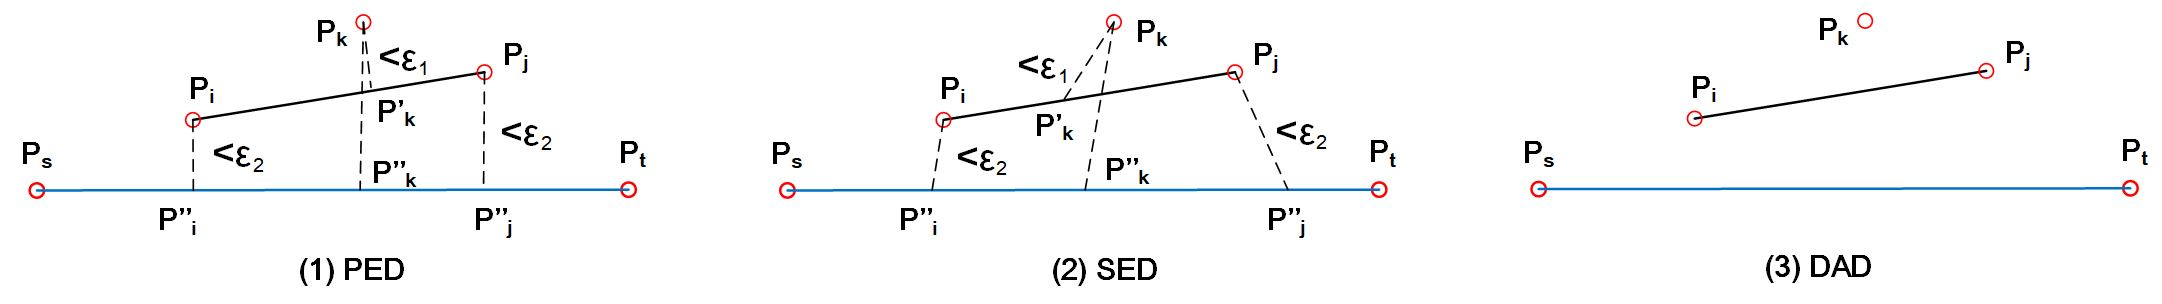
\includegraphics[scale=0.6]{Figures/Fig-aging-error.jpg}
	
	\caption{\small Examples of aging errors.}
	\vspace{-2ex}
	\label{fig:aging-error}
\end{figure}

\textcolor{blue}{By Propositions \ref{theo-aging-error-dp} and \ref{theo-aging-distance}, it is obvious that all the above algorithms have bounded errors in data aging,  which make us freely re-compress trajectories by any of these algorithm as long as we use the same distance metric.}}
